\subsection{Classes $\mathcal{P}$ et $\mathcal{NP}$}

\subsubsection{Problèmes de décision}
\label{sub:problemes_de_decision}

\begin{definition}{Problème de décision}{problème_de_décision}
  Un problème de décision est un langage $P\subseteq\Sigma^*$.
\end{definition}
\begin{remark}
    Chaque langage $P$ représente un problème dont la réponse est oui ou non, en l'identifiant à sa fonction caractéristique
    $\chi_P$ :
    \begin{equation*}
        \begin{aligned}
            \chi_P\; :\; \Sigma^* &\rightarrow \{0,1\} \\
            u &\mapsto \begin{cases}
                1 & \text{si } u \in P \\
                0 & \text{sinon.}
            \end{cases}
        \end{aligned}
    \end{equation*}
    Étant donné un mot $u\in \Sigma^*$, il faut décider si $u\in P$ ou non.
\end{remark}
\begin{example}
    Avec $\Sigma = \{0,1\}$,
    \begin{equation*}
        \text{PRIME} = \{10,11,101,111,\dots\} 
    \end{equation*}
    l'ensemble des nombres premiers en binaire.
\end{example}
Il est parfois compliqué de représenter un problème comme un langage, effectivement, comment faire pour :
\begin{itemize}[label=\textbullet]
    \item ENTRÉE : un graphe $G$ non dirigé et un entier $k\in\mathbb{N}$.
    \item SORTIE : $1$ ssi on peut colorier $G$ avec $k$ couleurs.
\end{itemize}
On pourrait représenter ceci avec l'alphabet $\Sigma = \{0,1,\#,\$$\} avec ($i,j$) chaque arête qui pourrait être codée par 
le mot $\overline{i}\#\overline{j}$ où $\overline{i}$ est le codage binaire du sommet $i$. La paire ($G,k$) pourrait se 
coder par le mot :
\begin{equation*}
    \overline{i_1}\#\overline{j_1}\$\overline{i_2}\#\overline{j_2}\$\cdots\$\overline{i_m}\#\overline{j_m}\$\overline{k}
\end{equation*}
\warningbox{Le codage peut influencer la complexité. Il sera parfois nécessaire de changer le codage pour obtenir une complexité 
plus faible.}

\subsubsection{Problème d'optimisation}
\label{sub:probleme_d_optimisation}
\begin{itemize}[label=\textbullet]
    \item Un problème d'optimisation est un problème où l'on souhaite maximiser/minimiser une certaine quantité.
    \begin{itemize}[label=$\rightarrow$]
        \item Trouver la longueur d'un plus court chemin entre deux sommets ($s$ et $t$) d'un graphe.
    \end{itemize}
    \item Un problème d'optimisation peut être associé à un problème de décision.
    \begin{itemize}[label=$\rightarrow$]
        \item Existe-t-il un chemin de longueur au plus $k$ de $s$ à $t$ ?
    \end{itemize}
    \item Si on sait résoudre le problème de décision, on peut parfois résoudre le problème d'optimisation.
    \begin{itemize}[label=$\rightarrow$]
        \item Pour trouver le plus court chemin de $s$ à $t$ dans un graphe à $n$ sommets, on peut faire une recherche
        dichotomique.
    \end{itemize}
\end{itemize}

\subsubsection{Algorithme de décision}
\label{sub:algorithme_de_decision}
\begin{definition}{Algorithme de décision}{algorithme_de_décision}
    Un problème $P\subseteq\Sigma^*$ est décidé par un algorithme $A$ si pour tout mot $u\in\Sigma^*$;
    \begin{itemize}[label=\textbullet]
        \item $A$ se termine et retourne 1 si $u\in P$.
        \item $A$ se termine et retourne 0 si $u\notin P$.
    \end{itemize}
    Un problème est décidable s'il existe un algorithme qui le décide.
\end{definition}

\subsubsection{La classe $\mathcal{P}$}
\label{sub:la_classe_p}
\begin{definition}{Classe $\mathcal{P}$}{classe_p}
    La classe $\mathcal{P}$ est la classe des problèmes pouvant être décidés en temps polynomial. Plus précisément,
    un problème $P\subseteq\Sigma^*$ est dans $\mathcal{P}$ s'il existe un algorithme $A$ et une constante $k$ tel que
    pour tout mot $u$ de longueur $n$,
    \begin{itemize}[label=\textbullet]
        \item $A$ retourne 1 en temps $O(n^k)$ si $u\in P$.
        \item $A$ retourne 0 en temps $O(n^k)$ si $u\notin P$.
    \end{itemize}
\end{definition}
\begin{example}
    Exemples de problèmes dans $\mathcal{P}$ :
    \begin{itemize}[label=\textbullet]
        \item décider si un tableau est trié.
        \item décider si un entier codé en unaire est premier (facile)
        \item décider si un entier codé en binaire est premier (difficile)
    \end{itemize}
\end{example}


\subsubsection{Algorithme de vérification}
\label{sub:algorithme_de_verification}
Un algorithme de vérification est un algorithme qui sur base d'une solution candidate à un problème de décision, décide si
cette solution est valide ou non.
\begin{definition}{Algorithme de vérification}{algorithme_de_vérification}
    Un algorithme de vérification pour un problème $P\subseteq\Sigma^*$ est un algorithme de décision (retournant 1 ou 0)
    $A$ prenant deux mots en argument, qui termine pour toute entrée, tel que:
    \begin{equation*}
        P = \{u\in\Sigma^* | \exists v \in \Sigma^*, A(u,v)=1\}
    \end{equation*}
    Lorsque $A(u,v)=1$, $v$ est appelé un certificat pour $u$.
\end{definition}

\subsubsection{La classe $\mathcal{NP}$}
\label{sub:la_classe_np}
La classe $\mathcal{NP}$ est la classe des problèmes pouvant être vérifiés en temps polynomial par un algorithme de vérification.
\begin{definition}{Classe $\mathcal{NP}$}{classe_np}
    Un problème $P$ est dans $\mathcal{NP}$ s'il existe un algorithme de vérification $A$ de complexité polynomiale en temps
    et une constante $k$, tels que pour toute entrée $u$, les deux afformations suivantes sont équivalentes:
    \begin{enumerate}
        \item $u\in P$
        \item il existe un certificat $v$ de longueur polynomiale dans $u$ (i.e. $|v| = 0(|u|^k$)) tel que $A(u,v)=1$.
    \end{enumerate}
\end{definition}
\begin{example}
    Exemples de problèmes dans $\mathcal{NP}$ :
    \begin{itemize}[label=\textbullet]
        \item décider qu'un ensemble de clauses est satisfaisable.
        \item voyageur de commerce : étant donné $n$ villes, les distances entre les villes et un entier $d$, on voudrait
        savoir s'il existe un cycle de longueur $\leq d$ passant par toutes les villes une et une seule fois
        \item coloriage de graphes : peut-on choisiir un graphe avec moins de $k$ couleurs sans que deux sommets aient la 
        même couleur ?
        \item tous les problèmes de la classe $\mathcal{P}$ sont dans $\mathcal{NP}$.
    \end{itemize}
\end{example}
\begin{remark}
    Tout problème $\mathcal{NP}$ peut être décidé par un algorithme de complexité exponentielle en temps car étant donné un mot
    $u$ en entrée, il suffit d'énumérer tous les certificats de longueur au plus $a\cdot|u|^k$ et d'appeler l'algorithme de 
    vérification. Pour SAT, par exemple, il suffit d'énumérer toutes les interprétations possibles et les tester, pour le coloriage,
    il suffit dénumérer tous les coloriages possibles et les tester.\\
    Il existe une \textbf{fameuse conjecture} en théorie de la complexité qui est la suivante : 
    \begin{equation*}
        \mathcal{P}\neq\mathcal{NP}
    \end{equation*}
    Autrement dit, on ne sait pas encore démontrer que vérifier une solution candidate en temps polynomial est plus puissant que
    trouver une solution en temps polynomial.
\end{remark}

\subsubsection{Temps non-déterministe polynomial}
\label{sub:temps_non_deterministe_polynomial}
La classe $\mathcal{NP}$ peut également être définie comme la classe des problèmes pouvant être décidés en temps polynomial
par un algorithme non-déterministe. Si la réponse au problème est oui, alors il existe une exécution de l'algorithme après 
laquelle l'algorithme répondra oui.
\begin{example}
    SAT, choisir aléatoirement une valeur de vérité pour chaque variable et vérifier en temps linéaire qu'elles satisfont
    la formule.
\end{example}

\subsubsection{Réductions, $\mathcal{NP}$-dureté et $\mathcal{NP}$-complétude}
\label{sub:reductions_np_durete_et_np_completude}
\begin{definition}{$\mathcal{NP}$-dur}{np-dur}
    Un problème de décision $P$ est $\mathcal{NP}$-dur si pour tout problème $P'$ de $\mathcal{NP}$ se réduit à $P$ en temps
    polynomial, i.e. qu'il existe un algorithme $T$ de complexité polynomiale en temps, qui transforme tout mot $u'$ en un 
    mot $T(u')$ tel que $u'\in P'$ ssi $T(u')\in P$.
\end{definition}
Un problème qui est dans $\mathcal{NP}$ et $\mathcal{NP-dur}$ est dit $\mathcal{NP}$-complet, ce sont les plus compliqués de
la classe $\mathcal{NP}$.
\warningbox{Un problème $P$ peut être dans $\mathcal{NP}$-dur sans être dans $\mathcal{NP}$.}

Pour démontrer que $P$ est dans $\mathcal{NP}$-complet, il faut:
\begin{enumerate}
    \item Démontrer qu'il est dans $\mathcal{NP}$.
    \item Démontrer qu'il est dans $\mathcal{NP}$-dur. Pour démontrer qu'un problème $P$ est $\mathcal{NP}$-dur, il faut
    partir d'un problème connu comme étant $\mathcal{NP}$-dur, qu'on réduit dans notre problème en temps polynomial. Le 
    premier problème $\mathcal{NP}$-dur est le \textbf{Théorème de Cook}.
\end{enumerate}
\begin{figure}[H]
    \centering
    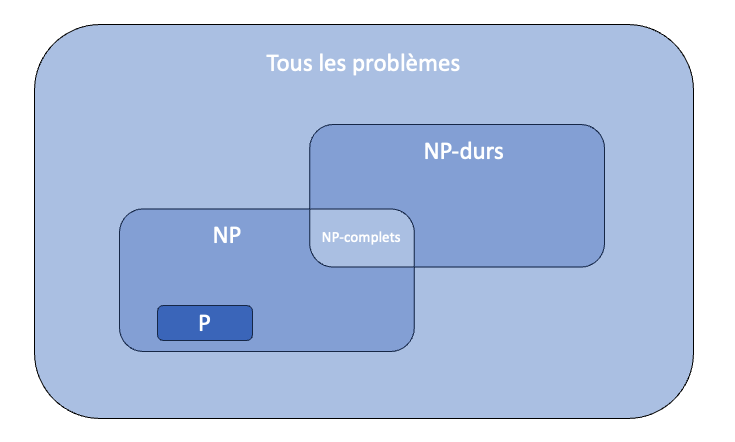
\includegraphics[scale=0.3]{pictures/NP.png}
    \caption{Relations entre les classes de complexité}
\end{figure}
\begin{theorem}{}{} 
    Si $\mathcal{P}\neq\mathcal{NP}$ et un problème $A$ est $\mathcal{NP}$-complet, alors $A\notin \mathcal{P}$.
\end{theorem}
\begin{proof}
    On va supposer que $A\in\mathcal{P}$ et en déduire la contradiction $\mathcal{P}=\mathcal{NP}$. On sait que $\mathcal{P}
    \subseteq\mathcal{NP}$, il nous reste à démontrer que $\mathcal{NP}\subseteq\mathcal{P}$. Soit $B$ un problème de 
    $\mathcal{NP}$ quelconque, montrons qu'il est dans $\mathcal{P}$. \\
    Comme $A$ est $\mathcal{NP}$-complet, $B$ se réduit à $A$ en temps polynomial. Comme $A\in\mathcal{P}$, nous avons un 
    algorithme en temps polynomial pour résoudre $B$ :
    \begin{itemize}[label=\textbullet]
        \item ENTRÉE : Instance $I$ de $B$
        \begin{enumerate}
            \item Transformer $I$ en une instance $I'$ de $A$ en temps polynomial. \textcolor{green}{$O(n^c)$}
            \item Résoudre $I'$ en temps polynomial. \textcolor{green}{$O(n^d)$}
        \end{enumerate}
    \end{itemize}
    Supposons que la réduction se fasse en temps $O(n^c)$ pour une constante $c$ et que $A$ se résout en temps $O(n^d)$ pour
    une constante $d$. Alors $B$ se résout en temps $O(n^{cd})$ :
    \begin{enumerate}
        \item Puisque l'étape 1 se fait en temps $O(n^c)$, où $n$ est la taille de $I$, la taille de $I'$ est en $O(n^c)$.
        \item L'étape 2 est appliquée sur une entrée de taille $O(n^c)$, donc elle prend un temps $O((n^c)^d) = O(n^{cd})$.
    \end{enumerate}
\end{proof}
\begin{lemma}{}{}
    Si vous prouvez qu'un problème $A$ est dans $\mathcal{P}$ et est $\mathcal{NP}$-complet, soit vous avez démontré 
    $\mathcal{P}=\mathcal{NP}$, soit vous avez fait une erreur.
\end{lemma}
\begin{lemma}{}{}
    Si vous ne trouvez pas d'algorithme en temps polynomial pour votre problème, alors peut-être qu'il est $\mathcal{NP}$-complet.
    et dans ce cas vous avez peu de chances d'en trouver un.
\end{lemma}

\subsubsection{Réduction de SAT vers 3-SAT}
\label{sub:reduction_de_sat_vers_3_sat}
\begin{theorem}{3SAT}{3sat}
    3SAT est $\mathcal{NP}$-complet.
\end{theorem}
\begin{proof}
    On doit démontrer que 3-SAT est dans $\mathcal{NP}$. On sait que SAT est dans $\mathcal{NP}$ et comme 3-SAT est Un
    cas particulier de SAT, on obtient que 3-SAT est dans $\mathcal{NP}$.
\end{proof}
\begin{remark}
    cf. le cours pour voir la réduction de SAT vers 3-SAT.
\end{remark}


\subsubsection{Bin Packing}
\label{sub:bin_packing}
Le problème du Bin Packing est le suivant : étant donné $n$ objets de poids $p_1,...,p_n$, peut-on les ranger dans $k$ boîtes
contenant au max $C$ kg ?\\

Ce problème est $\mathcal{NP}$-complet. Effectivement :
\begin{enumerate}
    \item BinPacking est dans $\mathcal{NP}$ : on peut vérifier en temps polynomial (une assignation de chaque objet à un numéro
    de sac entre 1 et $k$) si une solution candidate satisfait la contrainte de capacité.
    \item BinPacking est $\mathcal{NP}$-dur : Ceci est démontrable en faisant la réduction en temps polynomial du problème 2-
    partition, qui est un problème $\mathcal{NP}$-complet.
    \begin{proof}
        \begin{itemize}[label=$\rightarrow$]
            \item \textbf{Instance de 2-partition} : $n$ entiers $c_1,...,c_n$. On veut savoir s'il existe $S\subseteq\{1,...,n\}$
            tel que $\sum_{i\in S}c_i = \sum_{i\notin S}c_i$. Soit $S = \sum_{i=1}^{n}c_i$. On peut supposer que $S$ est paire sinon
            il n'y a pas de solution.
            \item \textbf{Réduction vers BinPacking} : On prend $C = S/2$ et les objets $1,\cdots,n$ de poids $c-1,\cdots,c_n$ et 
            $k=2$. Il y a une solution au problème 2-partition ssi il y a une solution au problème BinPacking. De plus, on peut 
            construire cette instance de BinPacking en temps polynomial. 
        \end{itemize}
    \end{proof}
    \item BinPacking est $\mathcal{NP}$-complet : on a montré qu'il est dans $\mathcal{NP}$ et $\mathcal{NP}$-dur.
\end{enumerate}
Il est également possible de montrer que GRAPHCOLOR est $\mathcal{NP}$-complet en réduisant le problème 3-SAT vers GRAPHCOLOR
en temps polynomial, pour voir ceci, voir le cours. (slides 25 jusqu'à 34)\\
\begin{remark}
    Il existe également d'autres classes de complexité comme PSPACE, EXPTIME, NPSPACE...
    Elles respectent les inclusions suivantes :
    \begin{equation*}
        \mathcal{P}\subseteq\mathcal{NP}\subseteq\text{PSPACE}\subseteq\text{EXPTIME}\subseteq\text{NEXPTIME}\subseteq\dots
        \subseteq \text{décidables}
    \end{equation*}
\end{remark}


\subsection{Problèemes indécidables}
\label{sub:probleemes_indecidables}
\begin{definition}{Problème indécidable}{problème_indécidable}
    Un problème de décision $P$ sur un alphabet $\Sigma$ est indécidable s'il n'existe pas d'algorithme $A$ prenant un mot sur
    $\Sigma$ et retournan, en un nombre fini d'étapes de calcul, la valeur 0 ou 1, tel que pour tout mot $x$ sur $\Sigma$,
    $A(x)=1$ ssi $x\in P$.\\
    En d'autres termes, un problème est indécidable s'il n'existe pas d'algorithme pour le résoudre.
\end{definition}

\subsubsection{Problème de l'arrêt}
\label{sub:probleme_de_l_arret}
\begin{minted}{python}
    while(True): print("hello")
\end{minted}
Ce programme ne s'arrête jamais.
\begin{definition}{Problème de l'arrêt}{problème_de_l_arrêt}
    \begin{itemize}[label=\textbullet]
        \item ENTRÉE : le code source d'un programme $P$ lisant des chaînes de caractères et une chaîne de caractères $x$.
        \item SORTIE : 1 ssi $P$ s'arrête sur l'entrée $x$, 0 sinon.
    \end{itemize}
\end{definition}
\begin{proof}
    On procède par l'absurde en supposant qu'il existe un programme HALT$(c_p,x)$ qui décide le problème de l'arrêt, pour tout
    programme $P$ donné par son code $c_p$ et toute chaîne de caractères $x$.\\
    À partir de HALT, on définit le programme PARADOX suivant :
    \begin{minted}{python}
    def PARADOX(c:string):
        if HALT(c,c): loop forever
        else: stop
    \end{minted}
    On appelle PARADOX($c_{\text{PARADOX}}$), où $c_{\text{PARADOX}}$ est le code source de PARADOX. On a deux cas :
    \begin{enumerate}
        \item Si PARADOX($c_{PARADOX}$) s'arrête, alors c'est que HALT($c_{PARADOX},c_{PARADOX}$) = 0, donc 
        PARADOX($c_{PARADOX}$) boucle infiniment.
        \item Si PARADOX($c_{PARADOX}$) ne s'arrête pas, alors c'est que HALT($c_{PARADOX},c_{PARADOX}$) = 1, donc
        PARADOX($c_{PARADOX}$) s'arrête.
    \end{enumerate}
    Dans les deux cas, on obtient une contradiction, donc le programme HALT ne peut pas exister.
\end{proof}

\subsubsection{Problème de la Correspondance de Post}
\label{sub:probleme_de_la_correspondance_de_post}
Soit $\Sigma = \{0,1\}$. Un mot $u$ sur $\Sigma$ est une séquence finie d'éléments de $\Sigma$. Deux mots $u$ et $v$ peuvent
être concaténés pour former un nouveau mot $uv$. L'élément neutre pour la concaténation est le mot vide $\epsilon$.\\
Par exemple : $u=01$ est un mot, $v=110$ est un mot, $uv=01110$, $\epsilon u=u\epsilon=u=01$.
\begin{definition}{Problème de la Correspondance de Post}{problème_de_la_correspondance_de_post}
    \begin{itemize}[label=\textbullet]
        \item ENTRÉE : $(u_1,v_1),\cdots,(u_n,v_n),n\geq 1, n$ paires de mots (possiblement vides) sur $\Sigma$.
        \item SORTIE : 1 ssi il existe une séquence finie d'indices $i_1,\cdots,i_k\in\{1,\cdots,n\}$ telle que $k\geq 1$ et
        \begin{equation*}
            u_{i_1}\cdots u_{i_k} = v_{i_1}\cdots v_{i_k}
        \end{equation*}
    \end{itemize}
\end{definition}
\begin{example}
    Voici quelques exemples de ce problème :
    \begin{itemize}[label=\textbullet]
        \item $(u_1,v_1)=(100,00)$, $(u_2,v_2)=(0,01)$, Solution (parmi d'autres) : $2,1$
        \begin{equation*}
            u_2u_1 = 0100 = v_2v_1
        \end{equation*}
        \item $(u_1,v_1)=(1,100)$, $(u_2,v_2)=(0,\epsilon)$, Solution : $1,2,2$
        \begin{equation*}
            u_1u_2u_2 = 100 = v_1v_2v_2
        \end{equation*}
        \item $(u_1,v_1)=(1,0)$, $(u_2,v_2)=(0,1)$, Solution (parmi d'autres) : Pas de solution
    \end{itemize}
\end{example}
\begin{remark}
    Résultat admis.
\end{remark}

\subsubsection{Prouver l'indécidabilité d'un problème}
\label{sub:prouver_l_indecidabilite_d_un_probleme}
\begin{itemize}[label=\textbullet]
    \item Pour montrer l'indécidabilité d'un problème de décision $P_1$, on peut partir d'un problème de décision $P_2$ connu
    indécidable et on montre l'existence d'un algorithme (réduction) qui pour toute instance $I_2$ de $P_2$ construit une instance
    $I_1$ de $P_1$ telle que $I_1$ a une solution ssi $I_2$ a une solution.
    \item De cette façon, on montre que $P_1$ est "aussi difficile" que $P_2$. S'il existait un algorithme pour résoudre $P_1$,
    alors cela nous donnerait un algorithme pour résoudre $P_2$ : appliquer la réduction puis l'algorithme pour $P_1$. Cela 
    contredirait le fait que $P_2$ soit indécidable, donc il n'existe pas d'algorithme pour résoudre $P_1$.
\end{itemize}
\begin{remark}
    La notion de réduction est la même que pour démontrer la NP-dureté d'un problème, à la seule différence qu'on ne demande pas
    que l'algorithme qui calcule la réduction se fasse en temps polynomial.
\end{remark}